\chapter{Commitment to openness}
\section{Open Access and its friends}
\lsp has a commitment to openness. This means that, beyond Open Access, we also use Open Source Software, and we make our workflows and organizational structure publicly available so that other projects can draw on our work. The licenses we use obey the Open Definition, meaning that everybody is always free to use our work if they attribute it properly.




\section{Tracking Progress}
\subsection{github}
A book is a complex document. Once your book is in final production mode, we use github to track versions and changes (\figref{fig:latex:github}). You can use github during the writing process as well (in fact, this will make the transition much smoother).

\subsection{Trello}
In order to keep things organized, we use Trello (\figref{fig:latex:trello}). Trello allows to distribute tasks such as bibliography update, proofreading, index creation and so on and keeps track of progress.

\begin{figure}
\caption{Github highlighting version history}
\label{fig:latex:github}
 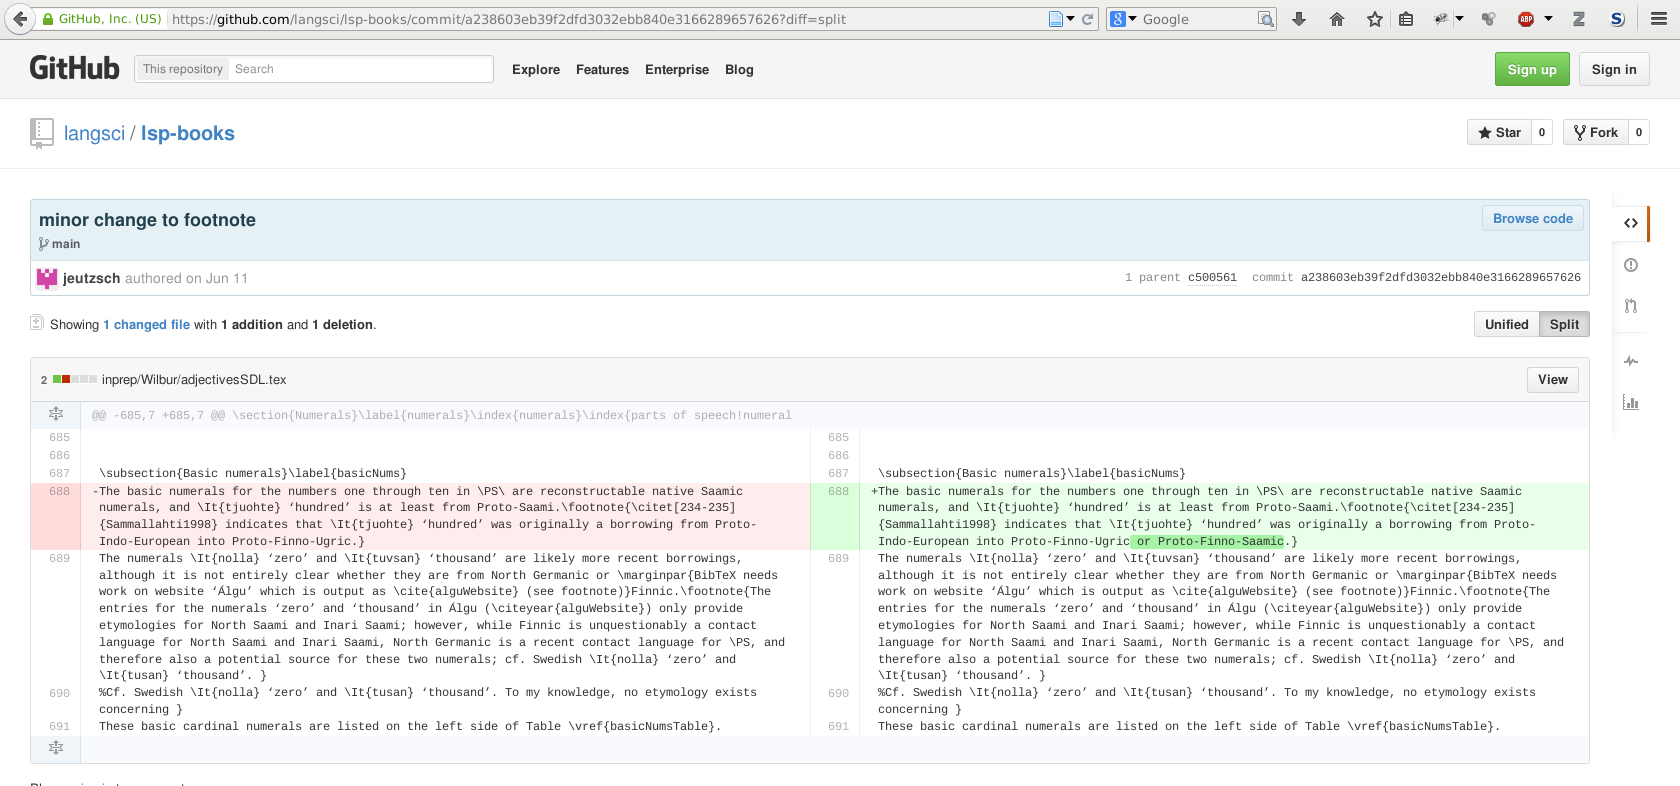
\includegraphics[width=\textwidth]{github.png}
\end{figure}

\begin{figure}
\caption{Trello}
\label{fig:latex:trello}
 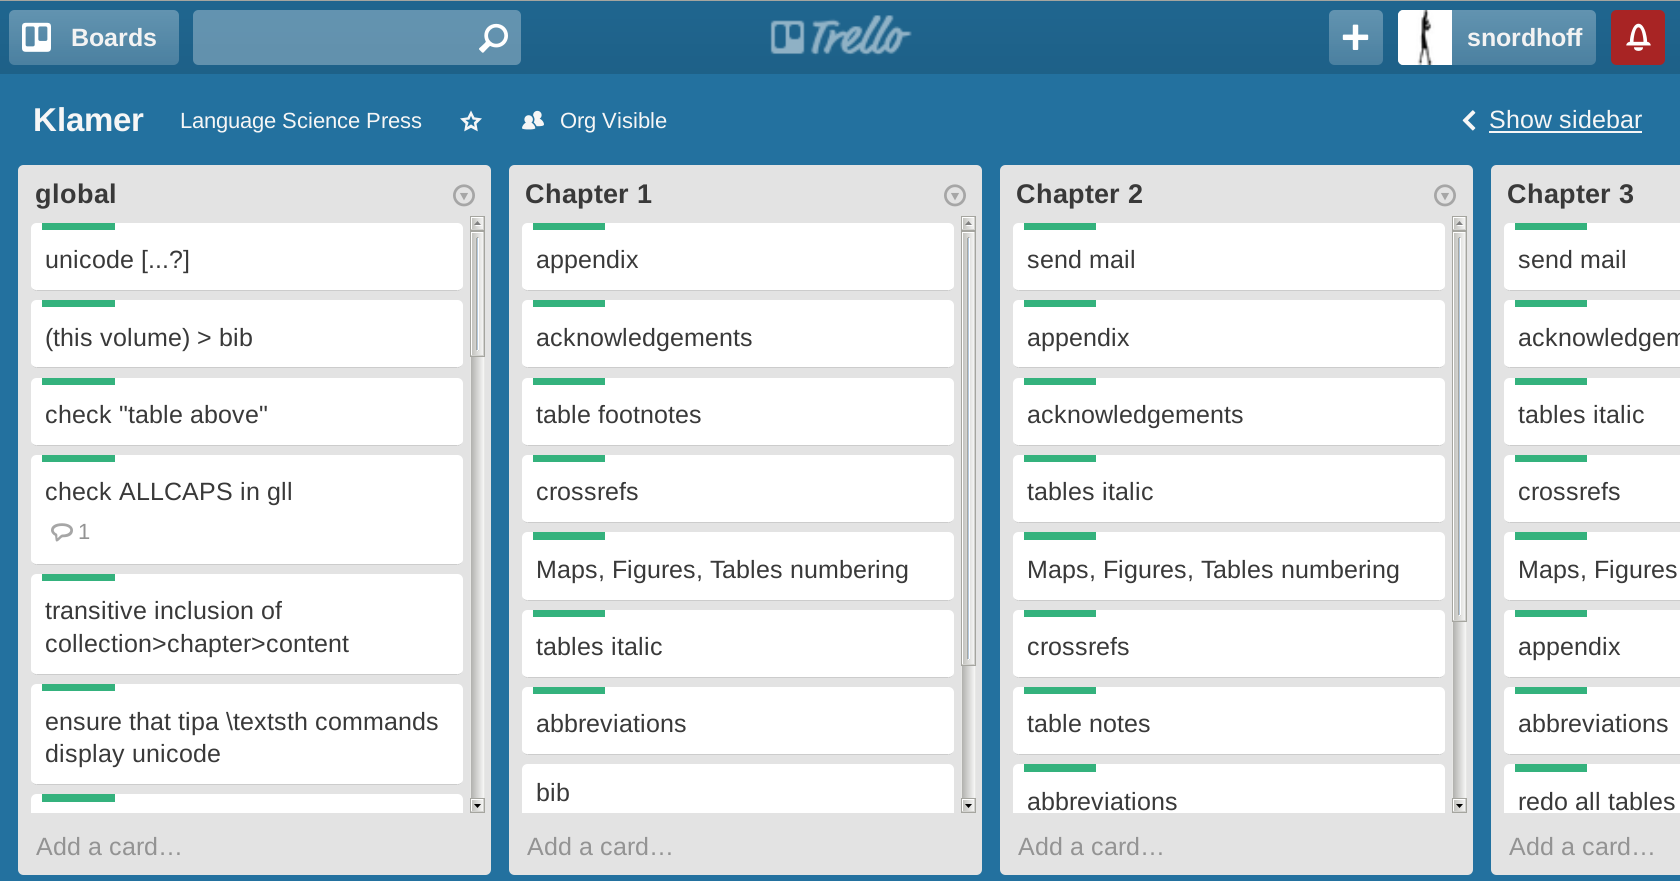
\includegraphics[width=\textwidth]{trello.png}
\end{figure}

